\documentclass[11pt, letterpaper]{article}

\usepackage[margin=1.2in]{geometry}
\usepackage{enumerate}
\usepackage{amssymb}
\usepackage{amsthm}
\usepackage{amsmath}
\usepackage{graphicx}
\usepackage{float}
\usepackage{wrapfig}
\usepackage{url}
%\usepackage{hyperref}

\newcommand{\includeCroppedPdf}[2][]{%
    \immediate\write18{pdfcrop #2}%
    \includegraphics[#1]{#2-crop}}

\newcommand{\CG}{\mathcal{G}}

\newcommand{\isom}{\cong}
\newcommand{\F}{\mathcal{F}}
\renewcommand{\H}{\mathcal{H}}
\newcommand{\B}{\mathbf{B}}
\newcommand{\CD}{\mathcal{D}}
\DeclareMathOperator{\Hom}{Hom}
\newcommand{\CH}{\mathcal{H}}
\newcommand{\R}{\mathbb{R}}
\newcommand{\s}{\mathbf{s}}
\newcommand{\grpd}{\rightrightarrows}
\renewcommand{\t}{\mathbf{t}}
\newcommand{\G}{\mathcal{G}}
\newcommand{\Z}{\mathbb{Z}}
\newcommand{\C}{\mathcal{C}}
\newcommand{\Q}{\mathbb{Q}}
\DeclareMathOperator{\Hol}{Hol}

\newtheorem{theorem}{Theorem}
\title{Research Statement}
\author{Joel Villatoro}
\date{}

\begin{document}
\maketitle
\section{Introduction}
Differential geometry is the study of calculus applied to smooth shapes called differentiable manifolds. The symmetries of such shapes are determined by mathematical structures known as Lie groups and Lie algebras. The core of my research program is to study such symmetries.

The two main recurring themes in my research are \emph{integration theory} and \emph{singular geometry}. 
In my context, integration theory refers to the study of the relationship between large scale (global) symmetries of an object and small scale (infinitesimal) symmetries. 
Singular geometry refers to the study of geometric objects which are \emph{a priori} poorly behaved but are constructed out of well behaved objects.

The main objects that appear in my research are Lie groups, Lie algebras, and their various generalizations. Lie groups are mathematical structures that represent the symmetries of geometric objects. On the other hand, Lie algebras represent the infinitesimal symmetries. Elements of a Lie algebra can be thought of as being ``derivatives'' of the elements of a Lie group. Roughly, integration theory studies the problem of whether one can can reconstruct a symmetry from its derivative. Singular geometry is the study of the types of spaces that occur when we chose to identify two different points related by a symmetry. For example, if one identifies the points in the plane that can be related by a half rotation, the resulting cone is singular space. 

The research projects I detail below include both long term projects(\ref{proj:non.integrable} and \ref{proj:noncommutative}) as well as some shorter term objectives(\ref{proj:holomorphic} and \ref{proj:vb.algebroids}).

The geometric nature of my work means that it provides a good foundation for the involvement of undergraduate, in addition to graduate, participation in my research program. 
Visualizations and research projects involving matrix groups and linearizable structures are simultaneously relevant to my interests and provide an excellent stepping stone for motivated undergraduates to enter the world of mathematical research.

In my research, I use diverse set of tools to investigate topics, including elements from algebraic geometry, category theory, symplectic geometry, and noncommutative geometry. My previous research projects have included both theory heavy \cite{MyThesis} as well as computational work\cite{Bpicpoiss}. Often, my work focuses on finding a new point of view on difficult problems. Let me give brief description of two such examples: 

Foliations are special kinds of partitions of manifolds obtained by constraining paths in the manifold to a set of allowed directions. An important invariant of a foliation is called the ``holonomy'' which measures the way that the foliation is twisted along a loop. Foliations can be classified as ``regular'' or ``singular'' with regular foliations being generally easier to study. Holonomy was first defined for regular foliations in terms of paths tangent to the allowed directions. For singular foliations, there are too many allowed directions and this flexibility meant that it was not known how to generalize this construction to the singular context. Eventually, Androilidakis and Skandalis\cite{AS.Holonomy},  gave a definition of holonomy for singular foliations but their approach was very different from the path-based approach of the regular case and the relationship between the two invariants was not obvious. In \cite{villatoro2019integration}, we developed a simpler path-based construction for the holonomy of a singular foliation that unified the regular and singular frameworks. 

The integration problem for Lie algebroids (a special kind of Lie algebra) is notorious for being very subtle and is known to be impossible in general\cite{almeida_suites_1985}. The problem that arises is that the ``integration'' fails to be a manifold. It was long been believed, but not known how, that it might be possible to fix this problem by permitting spaces slightly more general than a traditional manifold. In \cite{nonintegrable}, I showed that this is indeed true by developing a calculus for the types of singular spaces that integrate Lie algebroids.

\section{Background and preliminaries}

\subsection{Integration and differentiation}
Briefly, a Lie group \( G \) is just a group where \( G \) is equipped with the structure of a smooth manifold and the associated structure maps (multiplication and inverse) are smooth.

A Lie algebra is a vector space with a bi-linear operation:
\[ [\cdot , \cdot  ] \colon \mathfrak{g} \times \mathfrak{g} \to \mathfrak{g} \] 
which is anti-symmetric and satisfies the Jacobi identity.

There is a procedure which allows one to associate to any finite dimensional Lie group \( G \) a finite dimensional Lie algebra. This procedure is actually a functor:
\[ \mathcal{D} \colon \mathbf{LieGrp}  \to \mathbf{LieAlg} \]
from the category of finite dimensional Lie groups to finite dimensional Lie algebras. It is also possible to define this functor for many kinds of infinite dimensional Lie groups but the finite dimensional case is the most well-understood and illustrative.

Given a Lie algebra, \( \mathfrak{g} \) an \emph{integration} of \( \mathfrak{g} \) consists of providing a Lie group \( G \) together with an isomorphism \( \mathcal{D}(G) \cong \mathfrak{g}\). The foundation of integration theory can be summarized by the following theorem:
\begin{theorem}
The differentiation functor:
    \[ \mathcal{D} \colon \mathbf{LieGrp} \to \mathbf{LieAlg}\]
    with the following properties:
    \begin{itemize}
        \item (Lie's second theorem) If \( G \) and \( H\) are Lie groups where \( G \) is simply connected, then for every homomorphism of Lie algebras \( \phi \colon \mathcal{D}(G) \to \mathcal{D}(H) \) there is a unique homomorphism of Lie groups \( \Phi \colon G \to H \) such that \( \mathcal{D}(\Phi) = \phi\).
        \item (Lie's third theorem) If \( \mathfrak{g} \) is a Lie algebra, there exists a simply connected Lie group \( G \) such that \( \mathcal{D}(G) \cong \mathfrak{g} \).
    \end{itemize}
\end{theorem}
In other words, the integration problem for finite dimensional Lie groups and Lie algebras is completely solved. However, the situation is much more tricky if one generalizes by allowing infinite dimensional objects or extending the context to Lie \emph{groupoids}.

A groupoid is a generalization of the notion of a group where not all products are well defined. A groupoid \( \CG \) is determined by two sets \( \CG_1\) and \( \CG_0 \) called  the \emph{arrows} and \emph{objects}, respectively. To each arrow \( g \in \CG_1 \) we associate a source \( s(g)\) and target \( t(g)\) in \( \CG_0 \). When the source of \( g \in \CG_1 \) coincides with the target of \( h \in \CG_1 \) then we may take the product \( g \cdot h\).
As with groups, this operation is required to satisfy a few basic properties such as associativity, the existence of left and right units, and the existence of left and right inverses.

From this point of view, a group is just a groupoid where the set of objects \( \CG_0 \) is a single point (and therefore the product is defined for all pairs of arrows). Other examples of groupoids arise naturally from group actions, homotopy classes of paths, and germs of homeomorphisms between spaces.

A groupoid is called a Lie groupoid if the sets of objects and arrows are smooth manifolds and the structure maps are smooth. It is possible to extend the differentiation functor \( \mathcal{D} \) to Lie groupoids. However, rather than obtaining a Lie algebra, one obtains what is called a Lie algebroid.

Essentially, a Lie algebroid is a vector bundle over a smooth manifold that is equipped with a Lie algebra structure on its space of sections.

If we replace Lie groups with Lie groupoids and Lie algebras with Lie algebroids in the above theorem, we see that Lie's second theorem still holds\footnote{One must also slightly modify the condition of being ``simply connected''.} It was speculated, and even believed, for some time that Lie's third theorem was true as well. However, in 1985 Almeida and Molino\cite{almeida_suites_1985} produced an example of a non-integrable algebroid.

A breakthrough occurred for the integration problem when Cattaneo and Felder\cite{cattaneo_poisson_2001} introduced a new construction. This construction allowed one to associate a groupoid \( \mathcal{I}(A) \), commonly called the \emph{Weinstein groupoid}, to any Lie algebroid \(A \). The groupoid \( \mathcal{I}(A) \) is constructed by placing an equivalence relation on an infinite-dimensional space of paths. If the equivalence relation is sufficiently well behaved, the quotient space will be a smooth manifold and \( \mathcal{I}(A) \) is a Lie groupoid integrating \( A \).

Later, Crainic and Fernandes~\cite{Cint}, we able to study this equivalence relation in much more detail and establish a necessary and sufficient condition for the smoothness of \( \mathcal{I}(A) \). They also showed that \( A \) is integrable if and only if \( \mathcal{I}(A) \) is smooth.

\subsection{Morita equivalence and stacks}

Another major application for Lie groupoids is in the study of \emph{singular geometry}. In differential geometry, an object is said to be singular if the smooth structure of the object breaks down. Points where the smooth structure breaks down are called singularities. Examples of singularities in differential geometry include reflective boundaries, sharp edges, and changes in dimension. Even when one primarily deals with smooth, non-singular objects, singular spaces can still arise naturally. For instance, tilings of space can be classified by their associated orbifolds (an example of a singular space). 

A Lie groupoid can be regarded as an object that takes a smooth space and declares which points in space are considered equivalent. The geometric object one obtains by identifying equivalent points is an example of a singular space and it turns out that many natural examples of singular spaces can be seen as arising from Lie groupoids in this way. A consequence of this is that one can oftentimes use the language of Lie groupoids to adapt tools which were originally developed for smooth objects to the singular setting.

When we think of a Lie groupoid as representing a singular space, it is important to also have a notion of when two Lie groupoids represent the same singular space. This notion is called \emph{Morita equivalence}.

Geometrically, Morita equivalences arise from certain special kinds of actions of groupoids on a manifold. 
This is inspired by an analogy to the related notion of Morita equivalence in the context of algebras where Morita equivalences can be seen as arising from bimodules. 
These two notions of Morita equivalence are not only related by analogy. To any Lie groupoid one can associate a \( C^*\)-algebra and it was shown by Muhly et al~\cite{AlgebraMorita} that Morita equivalence of Lie groupoids implies (strong) Morita equivalence of the associated \( C^*\)-algebras.

Just as Morita equivalences of algebras give rise to equivalent categories of representations, Morita equivalences of groupoids give rise to equivalent categories of principal bundles. Given a Lie groupoid \( \CG \) let \( \B \CG \) denote the category of principal \( \CG \)-bundles. It turns out that \( \B \CG \) is more than just a category and it is a category theoretic object called a \emph{differentiable stack}.

The mapping \( \CG \to \B \CG \) gives rise to an equivalence of 2-categories between Lie groupoids and differentiable stacks. In particular, this means that if \( \G \) and \( \H \) are Lie groupoids with associated differentiable stacks \( \B \G \) and \( \B \H \), then \( \G \) and \( \H \) are Morita equivalent if and only if \( \B \G \) and \( \B \H \) are equivalent as stacks.

In practice, many naturally occuring Lie groupoids come with additional information such as Riemannian metrics, symplectic forms or complex structures. In such cases, it is desirable to study Morita equivalences which take into account this additional data. However, it is not always immediately obvious what it means for a Morita equivalence to be compatible with such geometries. Historically, the way such objects have been studied by geometers is via ad-hoc methods where the required equations and data are discovered by clever guesses guided by difficult to explain intuition. Examples of definitions developed in this way include Morita equivalence of Poisson manifolds\cite{MR1138048} and quasi-Hamiltonian actions\cite{MR1638045}. Generally speaking, the categorical side (i.e. the differentiable stack) is not well understood or even defined.

\section{Past Accomplishments}

\subsection{Integrating non-integrable algebroids}

As discussed in the background, not every Lie algebroid can be integrated by a Lie groupoid. For some time it has been conjectured one could resolve this issue using the notion of a diffeological space. Briefly, a diffeological space is a kind of generalization of the notion of a smooth structure allows us to talk about smooth functions even when the underlying space is highly pathological. Importantly, while the Weinstein groupoid \( \mathcal{I}(A) \) is not smooth, it does inherit a natural diffeological structure.

However, it is not so easy to use diffeology to resolve the issue. The main problem is that it is still not clear how to differentiate a diffeological groupoid. A few attempts (e.g. see \cite{androulidakis2020integration} and \cite{blohmann2023elastic}) had been made at some special cases but a differentiation theory general enough to capture non-integrable algebroids did not exist yet. 

In \cite{nonintegrable} I introduced a category of diffeological spaces called ``quasi-etale'' diffeological spaces.
Using the theory of quasi-etale diffeological spaces, I identified a class of diffeological groupoids called ``singular Lie groupoids'' and proved the following theorem.

\begin{theorem}[V.~\cite{nonintegrable}]
    There is a differentiation functor:
    \[ \mathcal{D} \colon  \textbf{SingLieGrpd} \to \textbf{LieAlg} \]
    from the category of singular Lie groupoids to the category of Lie algebroids. Furthermore, when \( \mathcal{D} \) is restricted to the subcategory of Lie groupoids, it coincides with the classical differentiation procedure.
\end{theorem}

\begin{theorem}
    The natural diffeology on the Weinstein groupoid \( \mathcal{I}(A) \) makes it into a singular Lie groupoid. Furthermore, \( \mathcal{D}(\mathcal{I}(A)) \cong A  \).
\end{theorem}

In other words, I showed that every Lie algebroid can be integrated as long as we consider the broader context of quasi-etale diffeological spaces and singular Lie groupoids. This resolves the most basic part (existence) of the integrability issue for Lie algebroids. However, there is more work to be done to develop a fully fledged Lie theory and this is the basis for (Project \ref{proj:non.integrable}).

\subsection{Poisson manifolds and their associated stacks}

Symplectic groupoids are a type of Lie groupoid that has been studied intensively. They are closely related to a class of geometric objects called Poisson manifolds. Poisson manifolds can be thought of as a geometric space in which there is a way of converting a measure of energy, represented by a Hamiltonian function, into dynamics. Just as Lie groupoids integrate Lie algebroids, symplectic groupoids integrate Poisson manifolds.

My work in \cite{dman} showed that it was possible to modify the construction of a differentiable stack from a groupoid so that it could take into account the symplectic part of symplectic groupoids. The main theorem can be summarized as follows:
\begin{theorem}[V.~\cite{dman}]\label{thm:dman}
Suppose \( \G \) and \( \H \) are \emph{symplectic} groupoids. Then there are stacks \( \B \G \) and \( \B \H \) associated to \( \G \) and \( \H \) with the property that \( \B \G \) and \( \B \H \) are equivalent as stacks if and only if \( \G \) and \( \H \) are symplectically Morita equivalent.
\end{theorem}
This work generated enough interest to earn me an invitation to speak at the 2018 edition of the Global Conference on Poisson Geometry, which is the premier research conference in this subject area. 

\subsection{Integration of singular foliations}
A singular foliation, intuitively, is a way of partitioning a geometric object into subsets called leaves. This is not unlike foliations in geology where a mineral exhibits a stratification into many thin layers. \emph{Regular foliations}, or sometimes just foliations, are foliations which the property that the leaves are all of the same dimension. The singular part of singular foliation is the presence of leaves of varying dimension.

Singular foliations appear in a variety of contexts in both pure and applied mathematics. Much of the early research into singular foliations was conducted by mathematicians researching control theory where it was realized that foliations formed a good mathematical model for the study of motion in robotics~\cite{narmanov2012foliation}.

% \addtocounter{footnote}{-1}
% \begin{wrapfigure}{r}{0.4\textwidth} 
% \centering
% 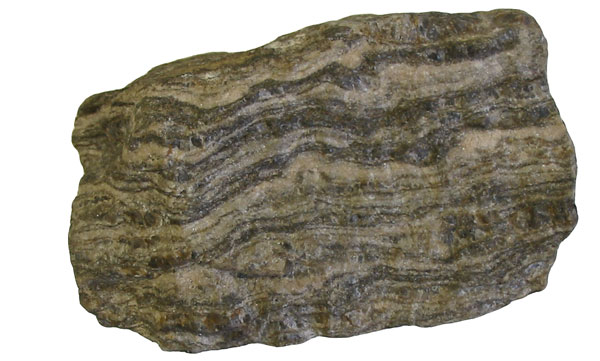
\includegraphics[width=0.3\textwidth]{Gneiss}
% \caption[Caption for LOF]{A real world example of a foliation. The leaves of a mathematical foliation are analogous to the different mineral strata.\footnotemark}
% \end{wrapfigure}
% \footnotetext{Photo by Siim Sepp and used under Creative Commons BY-SA 3.0. \url{https://commons.wikimedia.org/wiki/User:Siim}}

One of the most important invariants of a foliation is called its \emph{holonomy}. Intuitively, \emph{holonomy} measures the way the foliation twists along loops tangent to the leaves. When a foliation is regarded as an equivalence relation, the holonomy can be thought of as describing the naturally symmetries of the quotient space. 

Originally, this invariant was only understood in the context of regular foliations and it was unknown how to adapt the definition of holonomy to the singular case. A significant advance was made in \cite{AS.Holonomy} where Androilidakis and Skandalis managed to construct a groupoid from a singular foliation which was a clear analogue of the holonomy groupoid of regular foliation.

Although the Androulidakis-Skandalis holonomy groupoid bears a lot of similarities to an integration of some kind, it was constructed in a significantly different manner from the methods used by Crainic and Fernandes to study the integration of Lie algebroids. 

In \cite{villatoro2019integration}, Alfonso Garmendia and I successfully demonstrated a more natural path-based, construction of the holonomy groupoid of a singular foliation. The main theorem of our article can be roughly summarised by the following:

\begin{theorem}[Garmendia, V.\cite{villatoro2019integration}]\label{thm:sing.fol.paths}
Given a singular foliation \( \F \), there is a path based construction of another groupoid \( \Hol(\F) \). When the foliation is regular, this construction agrees with the classical holonomy groupoid of a singular foliation. Furthermore, in the singular case the groupoid \( \Hol(\F) \) is isomorphic to the holonomy groupoid of Androulidakis and Skandalis.
\end{theorem}

The key insight of this project was understanding the correct way to think about a singular foliation as a kind of generalized Lie algebroid. This suggested that many of our techniques could be extended to another more general class of Lie algebras called \emph{sheaves of Lie-Rinehart algebras}. In my most recent preprint\cite{fresh} I prove several useful results which clarify many properties of sheaves of Lie-Rinehart algebras.

\subsection{Picard groups of b-symplectic manifolds}
As mentioned in the introduction, two Lie groupoids defined to be Morita equivalent if they represent the same singular space. A closely related notion is the so called \emph{Picard group} of a Lie groupoid. The Picard group of a Lie groupoid is the set of all symmetries of the underlying singular space. The diversity of singular spaces means that the Picard group can range from massive and essentially incalculable to relatively small (even finite).

The notion of the Picard group for both Lie groupoids and Lie algebroids was initially introduced by Weinstein and Burstzyn in 2003~\cite{MR2074983}. Even today, computations of the Picard group are rather rare in the literature. In 2006 the first non-trivial computation of a Picard group was performed by Radko and Shlyakhtenko~\cite{picsurface}. They computed the Picard group of a class Lie groupoids that are associated to two-dimensional geometric objects called b-Symplectic Manifolds.

In 2016~\cite{bsymp} I expanded upon their result to encompass many more examples of arbitrary (even) dimension. The technique I used to solve this problem was to a decorated graph called a \emph{discrete presentation}. The discrete presentation is a sort of skeleton for a b-symplectic manifold which contains all of the data needed to construct the desired Morita equivalences.


\subsection{Thesis work}
Due to the complexity in the formal language for stacks in category theory, the work I did in \cite{dman} required a fairly significant amount of checking of details to be proved carefully. This was made all the more difficult by the fact that a complete proof for the original Lie groupoid case did not exist in the literature. 

For my thesis, I noticed that similar techniques to the one I used in \cite{dman} could likely be adapted to many more notions of Morita equivalence in the literature. However, proving each case individually would require a large amount of essentially redundant work. To alleviate this, I worked to identify the minimal ingredients needed for the theory relating groupoids and stacks.

The technique I used was to define the notion of a \emph{good site}. Intuitively, a \emph{site} can be thought of as a mathematical playing field in which one can do geometry. A good site is one which has the necessary features to admit a theory of groupoids and stacks. Although the full result is stated in more technical language, the main theorem of my thesis could be summarized as follows:
\begin{theorem}[V.~\cite{MyThesis}]\label{thm:thesis}
Suppose \(\mathcal{C} \) is a good site. Then from a groupoid \( \G \) in \( \C \) one can construct a stack \( \B \G \) over \( \C \). Furthermore, this construction yields an equivalence (2,1)-categories.
\end{theorem}
The main application of this theorem is that it us to study many examples of Morita equivalence simultaneously. For example, my work provides an immediate recipe for associating a stack to VB-groupoids~\cite{del_Hoyo_2018} as well as Contact groupoids~\cite{Contact_Red}. 
Furthermore, this agrees with the pre-existing definition of Morita equivalence of VB-groupoids which appeared in~\cite{del_Hoyo_2018}.

While this theorem provides a recipe for understanding the relationship between groupoids and stacks, it is not necessarily trivial to apply this recipe to every version of Morita equivalence which occurs in the literature. Care must be taken when finding the appropriate site for each context and there is more work to be done in this area (see Research objective~\ref{proj:holomorphic}).




\section{Research Objectives}

\subsection{Non-integrable Lie theory and Morita theory}\label{proj:non.integrable}

In \cite{nonintegrable}, I showed that the category of quasi-etale diffeological spaces provides a context where one is able to integrate all algebroids. The aim of this project would be to build on this work to develop a Lie theory and Morita equivalence that is adapted for non-integrable algebroids.

This project is more long term and open ended as there are many theoretical elements that would be of interest to develop here. One of them would be to prove Lie's second theorem for singular Lie groupoids. Recall that Lie's second theorem says the following:
\begin{theorem}
    If \( \CG \) and \( \CH \) are Lie groupoids and \( \CG \) is source simply connected, then for all morphisms of Lie algebroids \( \phi \colon \CD(\CG) \to \CD(\CH) \) there exists a unique morphism of Lie groupoids \( \Phi \colon \CG \to \CG \) such that \( \CD(\Phi) = \phi \).
\end{theorem}
In order to prove such a theorem for singular Lie groupoids, it will be necessary to make sense of what \emph{source simply connected} should mean in this context.
It will also require overcoming some technical difficulties with making sense of flows of vector fields on singular Lie groupoids.

In order to do Morita theory, it will be necessary to develop a theory of principal bundles, bibundles, and stacks which is adapted for singular Lie groupoids.
My work in \cite{MyThesis} lays out a good starting point for this.

One of the main motivations of this project is also to allow us to better understand non-integrable Poisson manifolds. Recall that the integration of a Poisson manifold is a \emph{symplectic} groupoid. Therefore, we will also need to develop a version of symplectic geometry for quasi-etale diffeological spaces.

\subsection{Non-commutative geometry of Lie algebroids}\label{proj:noncommutative}

Lie groupoids and non-commutative geometry are linked by the notion of a \( C^*\)-algebra. Such algebras can be considered as models for the ``functions'' on some non-commutative space. 
From the point of view of groupoids and Morita theory, we can think of the \( C^*\)-algebra of a groupoid as being the non-commutative ring of functions on the associated singular space.

Examples of non-commutative spaces that can be obtained this way include the \( C^*\)-algebra of a foliation and the non-commutative torus. More generally, given an integrable Lie algebroid, one can construct a \( C^*\)-algebra by integrating the algebroid.

However, as we have learned, the integration of an algebroid is a singular Lie groupoid rather than a Lie groupoid. Due to the fact that singular Lie groupoids are not Hausdorff, it is not possible to obtain a \( C^*\) algebra in the same manner as one would for a Lie groupoid.

In many ways, singular Lie groupoids are more akin to 2-groups which suggests that the appropriate algebraic structure to associate to them is something more analogous to a Hopf algebra or a quantum group. Intuitively, the non-commutative space of a singular Lie groupoid should be something like a non-commutative groupoid. 

Broadly, the aim of this project would be to make precise exactly what kind of non-commutative groupoids are associated to Lie algebroids. Success in this project would involve proving a version of the Muhly et al\cite{AlgebraMorita} which says something along the lines of ``Morita equivalences of singular Lie groupoids give rise to Morita equivalence of non-commutative grouoids.''

A potentially valuable tool here is the notion of a Hopfish algebra\cite{Hopfish}, although this object is not quite general enough for our purposes. Examining the objects involved reveals that the problem is essentially to find out what kind of algebraic object one should associate to a 2-groupoid and what is the appropriate notion of Morita equivalence. 

In a forthcoming article, in preparation, with Angel Roman, we will examine a few ways one can use representation theory and Hopf-like structures to better understand the algebraic properties of compact, strict 2-groups which are essentially a special case of singular Lie groupoids\cite{doublegrpds}.

\subsection{Stacks for holomorphic symplectic groupoids}\label{proj:holomorphic}
Apart from symplectic groupoids, the groupoid structures of greatest interest to those in the field are perhaps holomorphic symplectic groupoids. Holomorphic symplectic groupoids are similar to traditional symplectic groupoids but they come with additional geometry which makes them much more rigid.

The primary motivation for the study of such groupoids is in connection to a field known as generalized geometry. Generalized geometry and generalized complex structures~\cite{Hitchin,GCGualt} are a class of geometric structures with significant connections to symplectic geometry, Floer theory and string theory. Of particular note is their relationship to Branes which play a significant role in string theory, homological mirror symmetry and related models in theoretical physics (see, for example, Gukov and Witten\cite{GukovWitten}). In the context of holomorphic symplectic groupoids Branes appear as certain Lagrangian submanifolds of Morita equivalences\cite{BigBraneGualt} and therefore it is a topic of great interest to better understand Morita equivalence and stacks for holomorphic symplectic groupoids.

Due to the theoretical developments I made in \cite{dman} and \cite{MyThesis} the path forward here should be clear. One needs to weaken the non-degeneracy conditions on generalized complex structures and verify that the resulting structures constitute a sufficiently well-behaved site.

\subsection{Integration of LA-Groupoids}\label{proj:vb.algebroids}
Another notable class of generalized algebroid is that of LA-groupoids. Roughly speaking, an LA-groupoid is an object which is simultaneously a Lie algebroid and a Lie groupoid. These structures appear fairly naturally in the context of studying geometric structures on Lie groupoids. Furthermore, it is known that an LA-groupoid can be obtained by differentiating an object known as a \emph{double groupoid}.

One of the obstructions to the understanding of this problem is that it is not completely clear what is the correct notion of a source simply-connected double groupoid. To resolve this problem, I intend to use the notion a \emph{Haefligar-path} to adapt the integration procedure of Crainic and Fernandes to double groupoids.

There are some partial results. For instance, in a paper by Stefanini~\cite{Stefanini} a sufficient criteria for integrating LA-groupoids was obtained. While this is is progress, these conditions are much stronger than what is necessary. For example, by utilizing the conditions of Stefanini, it is not even clear that the tangent LA-groupoid of a Lie groupoid (one of the most basic examples) is integrable even though it admits an `obvious' integration.


\renewcommand{\refname}{References Cited}
\bibliography{articledb}
\bibliographystyle{plain}
\end{document}